\documentclass[a4paper,10pt]{article}
\usepackage[utf8]{inputenc}
\usepackage{graphicx,url}

%opening
\title{Gestão de Portfólio de Projetos}
\author{Ana Carolina Alves Rodrigues, Rodolfo Miranda de Barros}

\begin{document}

\maketitle

\begin{abstract}

\end{abstract}

\section{Introdução}
\flushleft
O desenvolvimento de projetos atualmente tem buscado soluções que auxiliem a demanda do mercado de forma que seus recursos possam ser aplicados
consistentemente, fazendo assim com que atrasos, desperdícios e prejuízos sejam minimizados de forma a obtenção de execuções otimizadas que propiciem maior e melhor retorno. 
Para isso busca-se utilizar ferramentas e técnicas que contemplem aspectos de eficiência (uso de recursos) e eficácia (obtenção de resultados positivos para a organização).
Dessa forma torna-se comum a utilização de técnicas como gerência de projetos e gerência de portfólio, essa segunda ainda pouco utilizada no Brasil.

\flushleft
Enquanto o gerenciamento de projetos ou programas está interessado em soluções que ``façam certo o trabalho'', a gestão de portfólio visa o ``faça o trabalho certo''.\cite{sppm} 
De forma a orientar a escolha pelos projetos que apresentem maior viabilidade para a instituição em relação as metas estratégicas existentes. No estudo ‘CHAOS Summary 2009’, 
o instituto de pesquisa Standish Group informa que houve uma queda nas taxas de sucesso dos projetos de TI. 
Pelo relatório, só 32\% das iniciativas são bem-sucedidas, ou seja, 68\% das atividades programadas pelo CIO e sua equipe acabam não atingindo os objetivos.

\flushleft
O propósito do processo Gerência de Portfólio de Projetos é iniciar e manter projetos que sejam necessários, suficientes e sustentáveis, de forma a atender
os objetivos estratégicos da organização, porém há pouco conhecimento sobre quais fatores da gestão de portfólio de projetos são específicos do contexto e quais são universais. 
Este processo compromete o investimento e os recursos organizacionais adequados e 
estabelece a autoridade necessária para executar os projetos selecionados.\cite{mps}


\subsection{Estratégia Organizacional}

O planejamento estratégico de uma organização tem como intuito definir objetivos para a seleção de programas de ação e execução, levando em conta as condições
internas e externas inerentes a instituição e a evolução almejada.No planejamento são definidos para que setores serão distribuídos os recursos existentes, de forma que os objetivos e metas traçadas sejam alcançados
ao longo do processo. É um planejamento global a curto, médio e longo prazo, que também  considera premissas básicas que deverão ser respeitadas pela instituição para que o processo tenha coerência e sustentação.

O planejamento estratégico deve comportar decisões sobre o futuro da organização, como:
\flushleft
\begin{itemize}	
\item[-] Objetivos organizacionais a longo prazo e seu desdobramento em objetivos	 departamentais detalhados; 
\item[-] As atividades escolhidas, isto é, os produtos (bens ou serviços) que a organização pretende produzir;
\item[-] O mercado visado pela organização, ou seja, os consumidores ou clientes que ela pretende abranger com seus produtos;
\item[-] Os lucros esperados para cada uma de suas atividades;
\item[-] Alternativas estratégicas quanto às suas atividades (manter o produto atual, maior penetração no mercado atual, desenvolver novos mercados);
\item[-] Interação vertical em direção aos fornecedores de recursos ou integração horizontal em direção aos consumidores ou clientes;
\item[-] Novos investimentos em recursos (materiais, financeiros, máquinas e equipamentos, recursos humanos, tecnologia etc.) para inovação (mudanças) ou para crescimento (expansão).
\end{itemize}
\flushleft
Ao término do planejamento estratégico a organização deve possuir missão, visão e valores bem definidos, a partir daí os projetos e processos da mesma
deverão ser desenvolvidos de acordo com estas definições, para que os objetivos e metas traçados possam ser alcançados e o planejamento bem sucedido.
\flushleft
Existe uma estimativa de que entre as 500 maiores empresas do mundo listadas pela Fortune de 50\% a 75\% delas têm suas principais estratégias ancoradas em projetos de TI.O que evidencia
a necessidade de técnicas e ferramentas que possam culminar no sucesso de tais estratégias. Um dos princípios da Gestão de Portfólio é exatamente alinhar o desenvolvimento
de projetos a estratégia organizacional traçada, fazendo assim com que todos os projetos tenham um objetivo em comum, traçado pela instituição, 
dessa forma a possibilidade de que o projeto seja abandonado ou acabe exaurindo os recursos da organização passa a ser insignificante. 


\subsection{A Gestão de Portfólio}
\flushleft
Define-se portfólio de projetos como sendo um grupo de projetos que serão conduzidos sob o patrocínio e/ou gerenciamento de uma organização particular.  
Ou ainda, um conjunto de projetos e/ou programas e outras atividades que são agrupados para facilitar o gerenciamento efetivo dos trabalhos para atingirem
os objetivos estratégicos do negócio.

\flushleft
Segundo o PMI ( Project Management Institute), portfólio pode ser definido como ``(...) um conjunto de projetos, programas e outros trabalhos que são agrupados para facilitar o gerenciamento efetivo daquele
trabalho para atender a objetivos estratégicos específicos. Os componentes do portfólio não necessariamente precisam ter alguma relação de dependência ou estar diretamente relacionados.``
Ainda segundo o PMI, projetos são definidos como ``esforço temporário empreendido para criar um único produto, serviço ou resultado``.
Os componentes de um portólio são quantificáveis, ou seja, eles podem ser medidos, classificados e priorizados.\cite{sppm}


\flushleft
Assim a gestão de portfólio consiste em técnicas para aprimorar a gerência de um conjunto de projetos ou programas de uma organização, esse gerenciamento
deverá ser feito de forma a tratar os projetos como um conjunto único, que esteja alinhado com a estratégia organizacional. A partir dessa gerência são acarretados diversos 
benefícios para a instituição, tais como: permitir a validação da estratégia corporativa; permitir o gerenciamento de recursos; ligar os resultados dos projetos com as estratégias organizacionais; manter a visibilidade de todas as informações vitais dos projetos; 
facilitar o acesso e as comunicações dentro da organização; subsidiar a tomada de decisões; dentre outros. A gestão trata-se em primeira instância, do afunilamento e canalização de todas as oportunidades de projetos que adentram a empresa para um processo de seleção, 
priorização e análise de viabilidade, objetivando criar uma carteira única de trabalho, mais alinhada às estratégias da empresa, que seja também mais transparente a todos os colaboradores e adaptada ao volume de recursos disponíveis.
Gerenciamento de portfólio consiste no gerenciamento centralizado de um ou mais portfólios  que inclui identificar, priorizar, autorizar, gerenciar, e controlar projetos, programas e outras atividades relacionadas, para atingir os objetivos estratégicos específicos do negócio.\cite{mps}

\begin{figure}
\centering
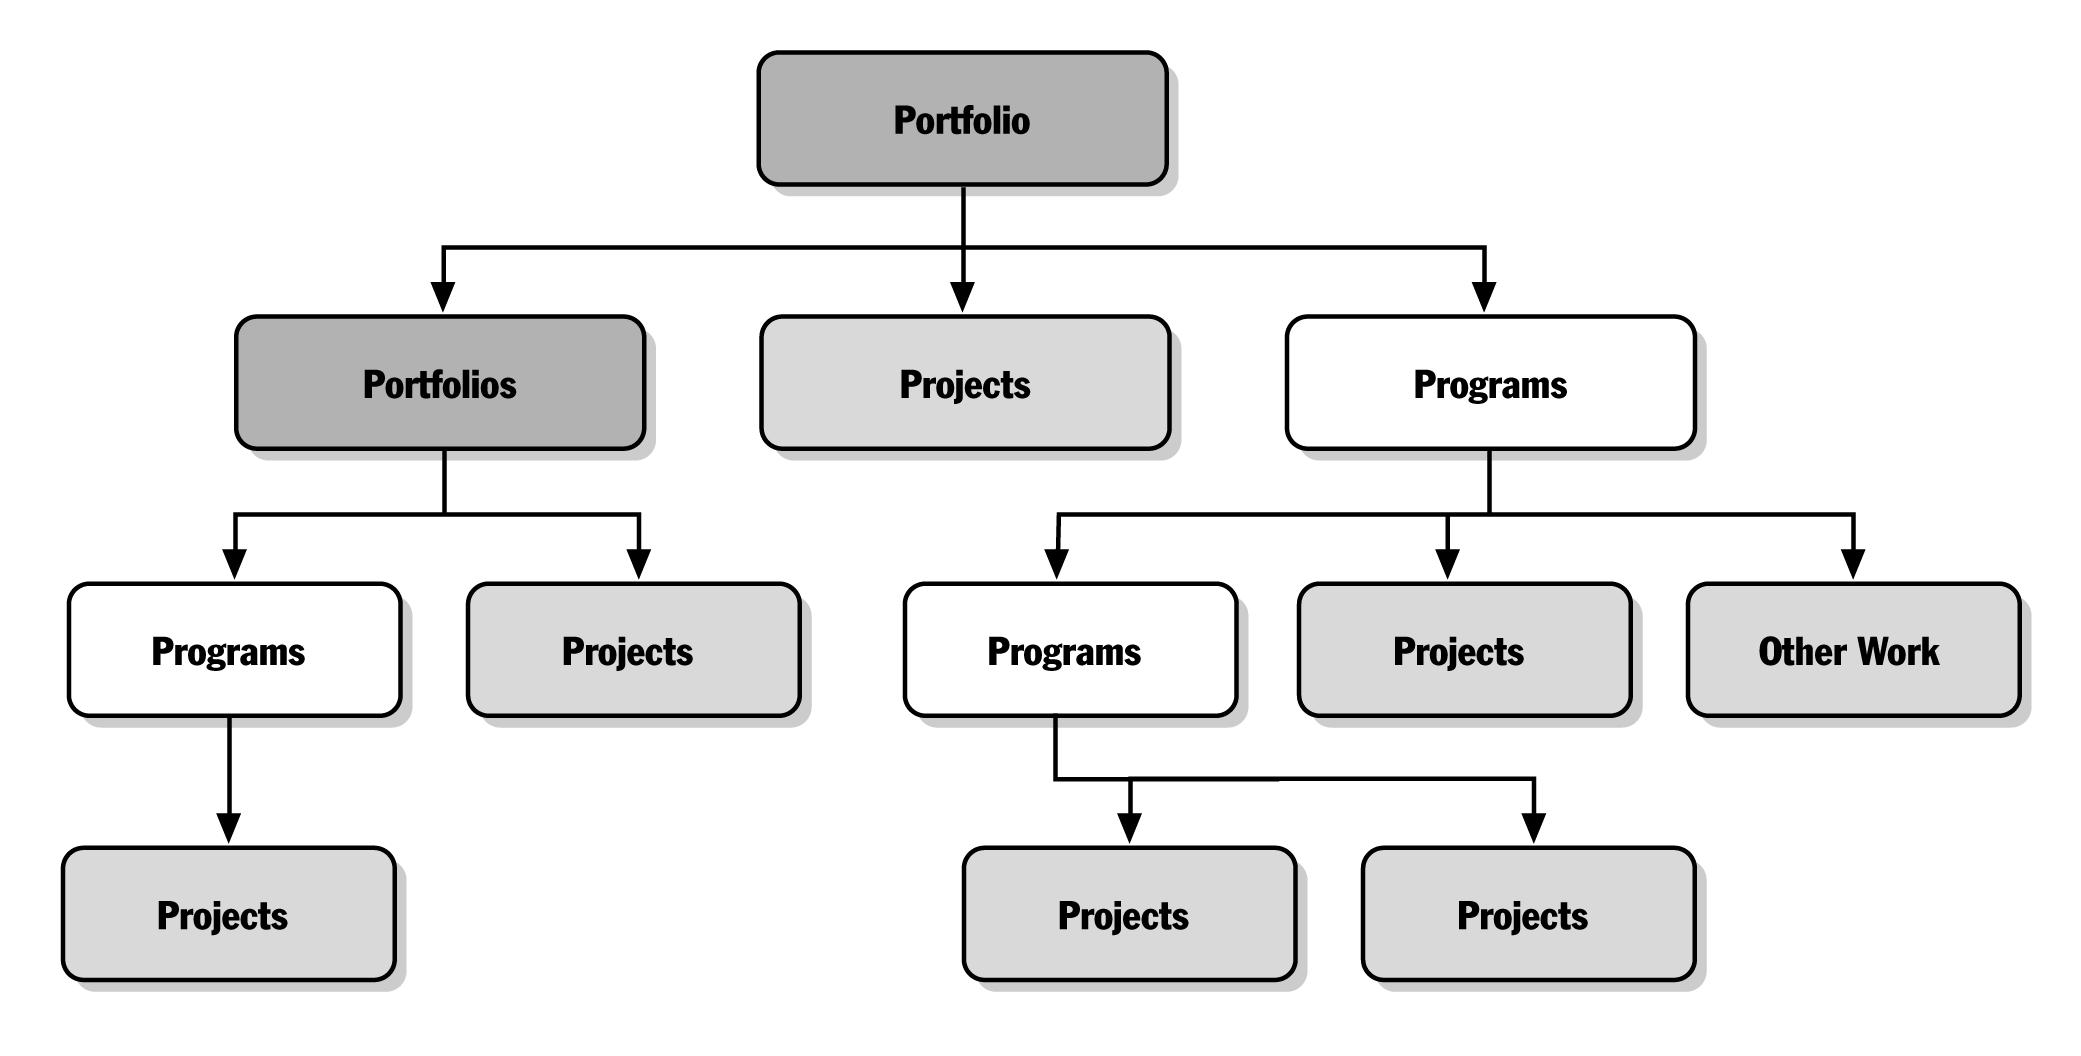
\includegraphics[width=.7\textwidth]{flow_sppm.jpg}
\caption{Exemplo dos relacionamentos de um Portfólio}
\end{figure} 

\flushleft

A Gerência de Portfólio de Projetos pode ser compreendida como a governança sobre o conjunto dos projetos. Ela atua em duas frentes: selecionando os projetos
que devem ser executados; e, uma vez em execução, avaliando se estes projetos continuam viáveis e aderentes aos critérios pelos quais foram aprovados.
O objetivo da etapa de seleção é criar uma combinação de projetos que melhor apóie os objetivos da organização, alinhada com as suas estratégias e com as
restrições de recursos (pessoas e orçamento) [LEVINE, 2005].

\flushleft
Apesar de não estar completamente ciente deste fato, toda organização pratica algum tipo de gestão de portfólio em seus projetos. Projetos são aprovados quase que rotineiramente e/ou em
momentos específicos dos ciclos de gestão das empresas. Gestão de projetos tornou-se, de fato, prática importante nos últimos anos com as organizações demandando profissionais certificados
com PMI e alocação de recursos para estruturas especializadas de projeto, como Project Management Offices. Muitas empresas, no entanto, organizam seus projetos de forma ad-hoc e
individualizada, com foco na determinação de prazos, realocação de recursos baseados em necessidades de curto prazo em constante mudança e soluções de disputas políticas sobre estes
recursos escassos.\cite{artigo}

\flushleft
Porém muitas organizações necessitam de um gerenciamento que seja capaz de integrar seu vasto número de projetos aos objetivos estratégicos traçados.
Neste momento é que se faz necessária a utilização de uma gestão de portfólio, que será responsável por ajudar as empresas a gerenciarem o conjunto (projetos e estratégia) como um todo,
de forma transparente e sistematizada. Para isso será necessária a utilização de métodos e práticas para priorizar e cancelar projetos, alocar recursos, definir responsabilidades,
fazer o gerenciamento dos riscos e definir se será necessário o engajamento de terceiros.

\flushleft
Para que a gestão seja utilizada de forma otimizada a organização deverá possuir um gerenciamento de projetos alinhado, de forma que seja possível obter os dados relevantes para a gestão, 
tais como: tempo de desenvolvimento, recursos utilizados, mão-de-obra, investimento, e demais informações inerentes ao desenvolvimento dos projetos da instituição. Ou seja, para que a gestão de portfólio funcione a organização precisa também de uma gestão de conhecimento atuante.
O conceito de projetos deverá estar bem definido, a forma como estes serão e são realizados, para que seja possível estimar o volume adequado de trabalho, sem esquecer que estes sempre deverão estar
atrelados a estratégia vigente e à disponibilidade de recursos. Além disso será necessário difundir junto aos membros da organização a cultura de utilização dessas não tão novas metodologias, já que 
estes serão os responsáveis por fazer com que o processo como um todo funcione.

\subsubsection{Benefícios da Gestão de Portfólio}
\flushleft
Existem diversos benefícios em se utilizar a gestão de portfólio, como já citado, a mesma provê uma visão mais ampla de todos os projetos da instituição e a situação em que estes se encontram.
A ferramenta utilizada para o controle da gestão pode ainda trazer outras informações que também necessitam ser avaliadas pelos altos executivos da organização nas tomadas de decisão quanto a manter
ou não um projeto e ainda as prioridades referentes a escolha.

\flushleft 
Entre os principais benefícios da gestão de portfólio podemos citar:\cite{atila}

\begin{itemize}
 \item Eliminação de projetos duplicados. Projetos idênticos, ou muito similares, sendo conduzidos em duas ou mais áreas na empresa podem ser fundidos em um só, reduzindo custos e evitando incompatibilidades no futuro.
 \item Combinação de projetos gerando economias de escala. Projetos que, embora não sejam idênticos, fazem sentido de serem executados juntos, pela mesma equipe e próximos no tempo. Um exemplo seriam projetos que produzem muitas entradas um para o outro.
 \item Visão clara da interdependência entre projetos. É mais fácil perceber quais saídas do projeto A devem ser entradas para o projeto B e vice-versa.
 \item Orienta a coordenação no tempo de diferentes projetos: o que deve acontecer no projeto A antes que se possa executar a tarefa X no projeto B.
 \item Redução da prioridade de projetos necessários, mas menos importantes ou urgentes. Ao comparar o escopo do projeto com as necessidades estratégicas da organização, é possível detectar quais projetos podem ser deixados para depois, quando houver mais recursos disponíveis.
 \item Aumento da prioridade de projetos estratégicos, mas de baixa visibilidade. Da mesma forma, o exame da relevância do projeto para o cumprimento das metas estratégicas pode levar à priorização e alocação de recursos adicionais a um projeto cuja visibilidade esteja baixa, 
talvez por falta de patrocinadores poderosos.
 \item Otimização da alocação de recursos e talentos. A Gestão de Portfolio de Projetos provê orientação na formação de equipes, usando as habilidades das pessoas onde contam mais. Se existe alguém na organização que é um expert em uma das fases-padrão dos projetos normalmente 
executados, por que esta pessoa deveria estar “fixa” em uma equipe que pega um projeto após o outro, participando também das atividades nas quais não é tão bom assim? Se João é um ótimo especificador de requisitos, mas um desenvolvedor apenas mediano, que sentido tem ele fazer 
tudo na equipe? Não é melhor que ele especifique os requisitos no projeto A, depois vá fazer o mesmo no projeto B e assim por diante? Com a visão global que a Gestão de Portfolio dá, é possível planejar melhor o emprego dos especialistas nos diversos projetos.
\end{itemize}

\subsubsection{Desafios da Gestão de Portfólio}
\flushleft
Apesar de ser aparentemente simples integrar os projetos e processos da organização as metas estratégicas traçadas, a gestão de portfólio encontra alguns desafios. O grande desafio encontrado
é no que diz respeito a priorização dos projetos. A maneira como será definido para qual projeto determinados recursos deverão ser alocados, levando em conta a existência de recursos escassos, ou seja, como dividir tais recursos
entre os projetos existentes.
No caso de empresas que desenvolvem projetos de software, um dos grandes desafios para
a gestão de portfólio de projetos é a caracterização de um projeto no que tange à definição de
critérios que realmente auxiliem na definição do valor do projeto para a organização.
Outro grande desafio encontrado diz respeito a tomada de decisão  sobre os investimentos, levando em consideração novamente a escassez de recursos e as necessidades estratégicas da organização. Ainda podemos
colocar o balanceamento do portfólio como desafio final, ou seja, uma metodologia que consiga desenvolver uma prática balanceada para a escolha do investimento ideal entre o risco do portfólio e
o retorno, a manutenção necessária e o crescimento alcançado, projetos curtos e projetos longos.\cite{cooper}

\section{Modelos de Gestão de Portfólio}
\flushleft
A elaboração de um modelo para gestão de portfólio de projetos deve levar em conta os principais desafios apresentados para a questão e uma solução para tais.
Caso essas questões não sejam observadas e estudadas, o modelo proposto poderá pender para um ou outro benefício da gestão, o que não resolverá o problema como um
todo e será apenas mais uma alternativa e não uma solução de fato. Para ilustrar alguns dos problemas que deverão ser sanados pelo modelo de gestão de portfólio podemos
citar: falta de alinhamento estratégico; baixa qualidade da carteira; faltas de critérios formais; interdependência 
técnica / comercial, entre outros \cite{martino1, martino2, cooper}.

\subsection{Modelo de Rabechini, Maximiano e Martins}
\flushleft
Um modelo de seis dimensões a ser utilizado por profissionais e demais interessados em gerenciamento de projetos, com ênfase
em portfólio, tem papel fundamental na difusão de práticas gerenciais nas organizações, apesar de sua característica abstrata e não tangível.\cite{rabechini}

\flushleft
A primeira das seis dimensões diz respeito à preparação do processo para o gerenciamento de portfólio. Nesta dimensão o fator preponderante  
é o planejamento estratégico da organização e que as metas e objetivos traçados estejam claros para o alto escalão da organização, 
pois estes serão os responsáveis por delinear o contexto estratégico e explorar o planejamento de forma a adequar o portfólio as estratégias traçadas. 
É preciso que os interessados conheçam de forma ampla o modelo de negócio para poder enquadrar os projetos e avaliá-los
corretamente, quando necessário.\cite{rabechini}

\flushleft
Ainda nesta dimensão, além da necessidade de entendimento dos elementos estratégicos, se faz necessário
a exploração do conhecimento das metodologias utilizadas para a avaliação dos projetos. Ou seja, será necessário
que os interessados na gestão de portfólio de projetos possuam conhecimento de quais os procedimentos a serem obedecidos
e as considerações de negócios que circundam todos os projetos existentes na organização.

Este processo deve contemplar os seguintes elementos:\cite{rabechini}

\begin{itemize}
 \item[a)] Identificação dos critérios de avaliação – neste elemento
os administradores da organização devem mostrar claramente seus objetivos e o gerente de portfolio deverá
entender os aspectos e indicadores pretendidos pela alta
administração.
\item[b)] Estabelecimento de pesos para tais critérios – neste elemento espera-se ter graus para diferenciar a importância
de cada critério, levantado anteriormente.
\end{itemize}

\flushleft
Ao término da primeira dimensão, o organização deverá notar um grande avanço na gestão de portfólio no que diz respeito
a estruturação de sua carteira de trabalho ( os projetos do portfólio ). Sendo assim a segunda dimensão, que diz respeito a 
identificação de projetos, poderá ser considerada.

\flushleft
Tendo em vista levantar todas as iniciativas, das áreas individuais da organização, para
que possam ser reunidas de forma coerente e consistente, a segunda dimensão tem como intuito a consideração
das informações mínimas sobre os projetos. Neste momento cabe a cada área fornecer justificativas e informações
sobre seus projetos para que estes possam ser considerados como parte do portfólio. Podem ser apresentados documentos
contendo informações como riscos, custos, prazos e outras informações inerentes a tal projeto. Porém as informações prioritárias
dessa dimensão são: objetivo, valores de prazo e custo, premissa para serem realizados com sucesso, indicadores a serem alcançados, 
restrições envolvidas e riscos que porventura possam ocorrer durante sua execução. A saída da segunda dimensão será uma lista de projetos.

\flushleft
Em posse da lista de projetos da dimensão anterior, é possível dar início a dimensão seguinte, que diz respeito a avaliação. Nesta dimensão
o intuito é definir uma nova lista, porém dessa vez com os projetos priorizados, ou seja, estes deverão receber notas, essas atribuidas de acordo com
os critérios definidos na primeira dimensão, agregando assim valor aos projetos. Para isto deve-se inicialmente
proporcionar a realização de rodadas de avaliação – aqui se espera ter elegido os avaliadores credenciados pela
organização e com eles estabelecer as notas para cada critério, projeto a projeto. Os conceitos de avaliação de
portfólio desenvolvidos por \cite{cooper} foram denominados de – Stage and Gate – e constituem a base para o desenvolvimento das avaliações aqui citadas.


\begin{figure}[ht]
\centering
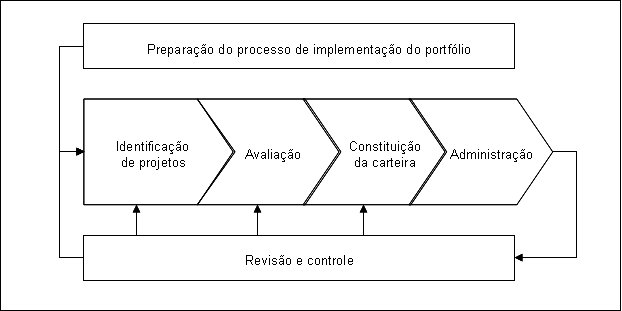
\includegraphics[width=.7\textwidth]{rabechini.jpg}
\caption{Modelo Rabechini, Maximiano e Martins}
\label{fig:exampleFig1}
\end{figure}

\flushleft
Nas rodadas de avaliação será possível estabelecer as informações de cada projeto e assim apresentar ao final informações que serão
utéis para a análise preliminar do portfólio. Nessa dimensão um aspecto importante que deverá ser levado em conta serão as ``linhas de corte''
para os projetos, pois nesse momento já é possível identificar as barreiras de cada projeto individualmente. Ou seja, ao término das avaliações
os projetos que ainda estão presentes serão os candidatos para a formação do portfólio.

\flushleft
A próxima dimensão, constituição da carteira, tem o intuito de estabelecer
um plano de gerenciamento de portfólio. O estabelecimento de prazos é recomendado por \cite{clark}, prazos estes
que devem ser de até um ano para alocação de recursos. Neste modelo é considerado que a dimensão atual deverá também
ser precedida de um plano agregado do portfólio, pois nessa dimensão o aspecto de maior importância deve-se a observação de que
neste momento serão selecionados os novos projetos que farão parte do portfólio e haverá então a disputa pelos recursos disponibilizados pela organização.

\flushleft
Na quinta dimensão, administração, constituiu-se a partir do modelo de \cite{crawford} quando esse se refere ao
aspecto do gerenciamento. Os elementos inerentes a esta dimensão são: 
o controle dos recursos aos diversos projetos em curso, o acompanhamento do ciclo de vida, projeto
a projeto, os custos e cronogramas financeiros e a qualidade do portfólio. Além destes elementos, nesta dimensão,
espera-se que os interessados possam administrar as competências dos recursos humanos através de capacitação, 
treinamentos e coaching, quando necessário, uma vez que o sucesso da carteira depende do desempenho destes.

\flushleft
Ao final, temos a sexta dimensão, que diz respeito a revisão e controle. Tendo em vista que os projetos já foram selecionados,
já existe a gerência do portfólio, cabe ao gerente de portfólio revisar o mesmo e acompanhar o desenvolvimento dos projetos. A metodologia
para o acompanhamento pode ser através de reuniões com os gerentes de projetos ou alguma outra forma instituída pela organização. Cabe aos
gerentes de projeto fornecer segundo a metodologia de gerência de projetos adotada pela organização, os indicadores de andamento de cada projetos
A partir daí, o gerente de portfólio será capaz de tomar decisões sobre a manutenção do portfólio.

\subsection{Modelo de gerenciamento de portfólio do PMI}
\flushleft
Em sua segunda edição do padrão para o gerenciamento de portfólio, o PMI apresenta uma a descrição de conhecimentos e práticas de gerenciamento de portfólio
aplicavéis e de reconhecida utilização. O padrão apresentando baseia-se no estabelecimento de processos, processos esses que deverão possuir uma 
sequência lógica de realização e agrupamento  por similaridade de função, além de serem divididos por áreas de conhecimento. \cite{sppm}

\flushleft
No modelo apresentado pelo PMI são definidos grupos de processos para o gerenciamento, os grupos aqui são definidos como
de alinhamento e de monitoramento e controle. Os processos do primeiro grupo, alinhamento, são os responsáveis por disponibilizar as informações, 
levando em consideração as metas traçadas no planejamento estratégico, é responsável ainda pelo estabelecimento de regras para avaliar seus componentes. 
São determinados como os componentes serão identificados, categorizados, avaliados, selecionados e incluídos no portfólio.

\flushleft
Já o segundo grupo, monitoramento e controle, fica responsável por reunir as atividades necessárias assegurando que o portfólio
esteja com um desempenho geral suficiente, fazendo assim com que seja possível atingir as metas traçadas no planejamento estratégico. Neste grupo, 
os processos serão responsáveis por revisar periodicamente os indicadores estabelecidos e verificar os benefícios que os componentes do portfólio estão agregando a organização.

\begin{figure}
\centering
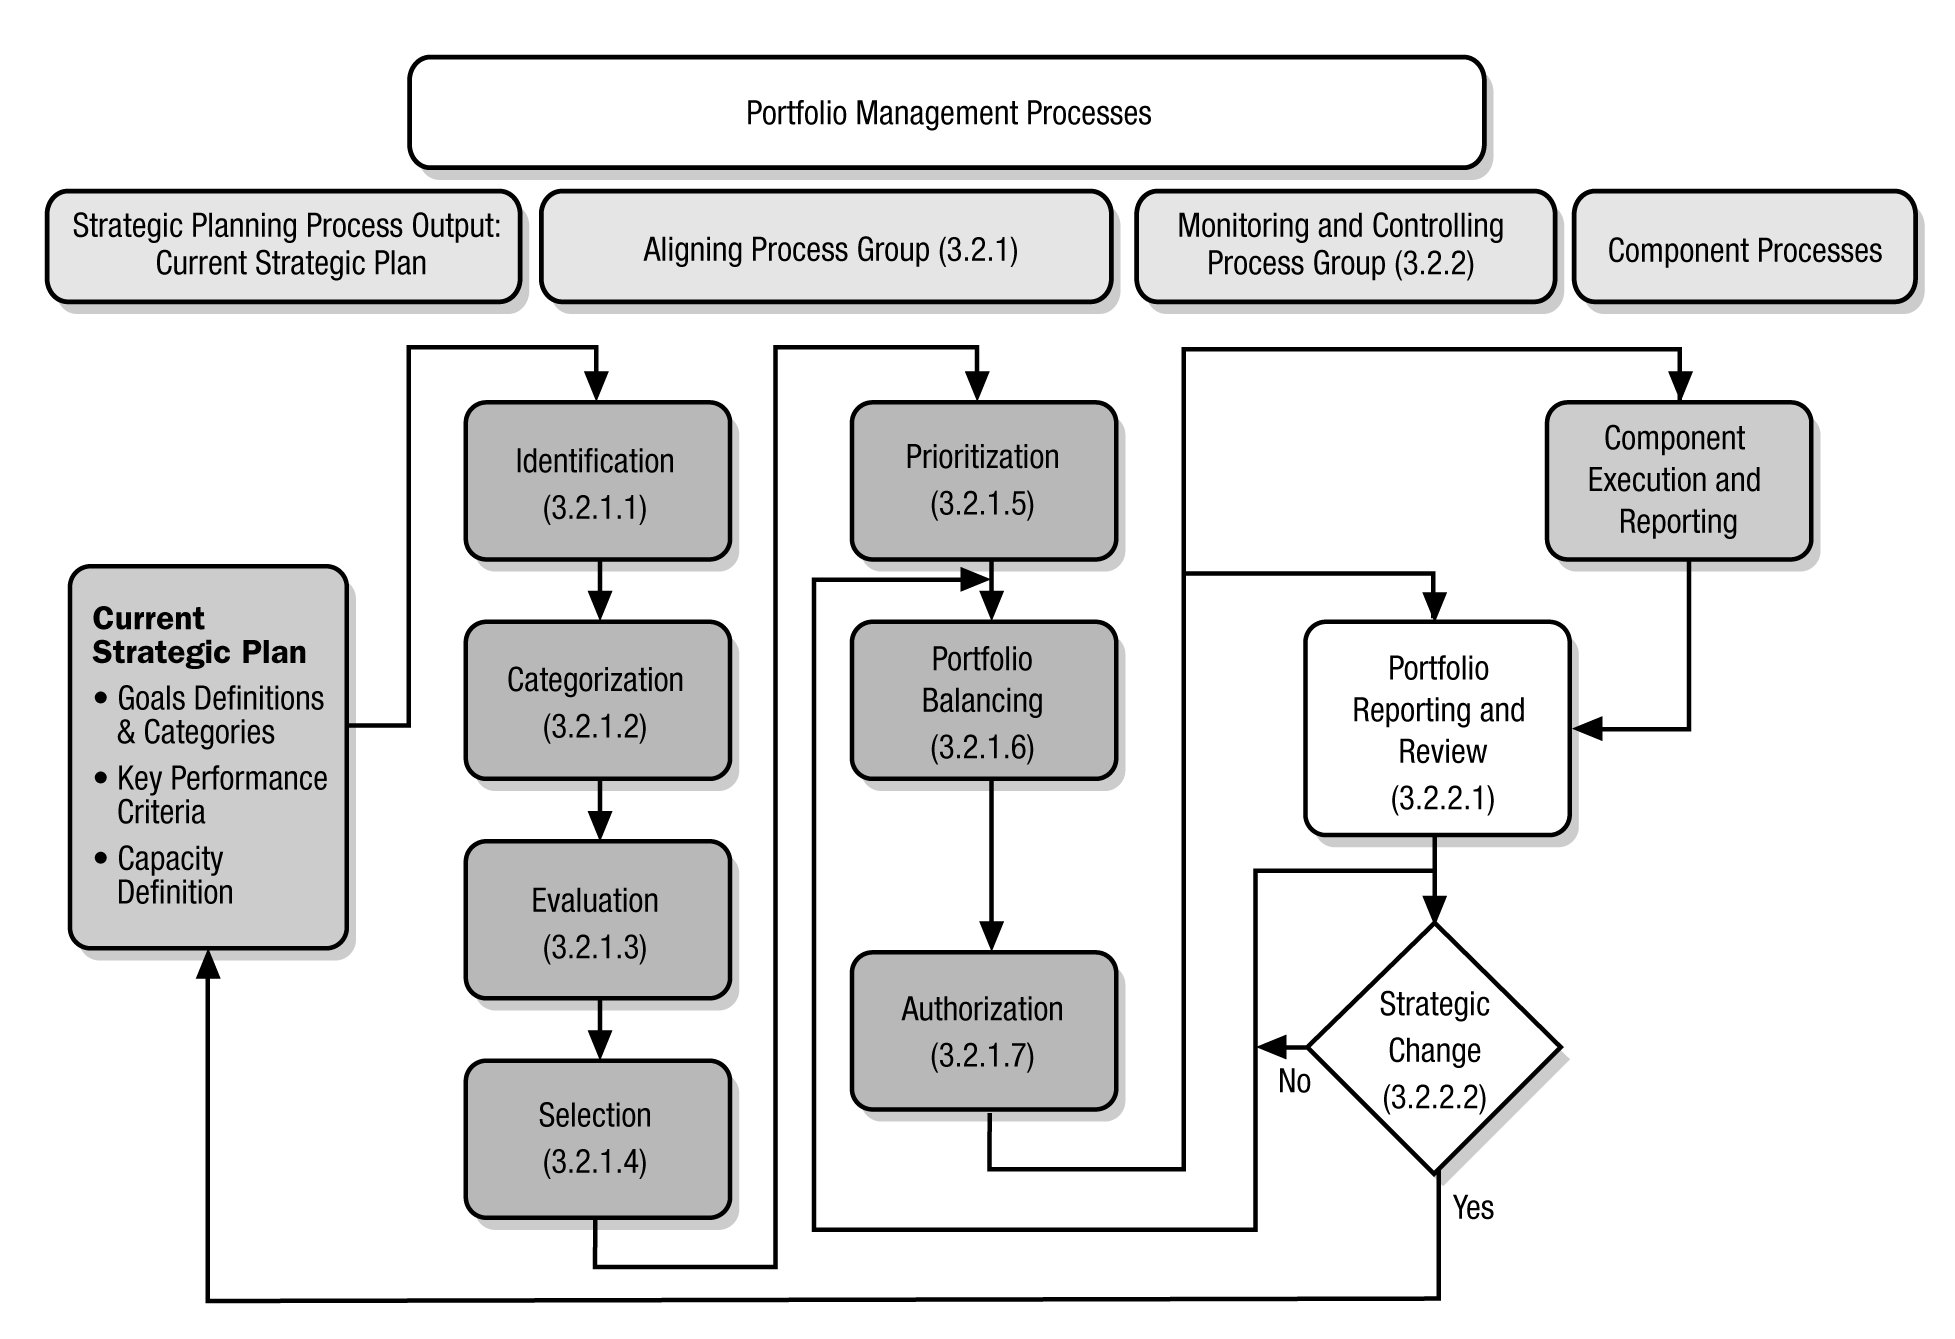
\includegraphics[width=.7\textwidth]{modelo_pmi.jpg}
\caption{Processos do gerenciamento de portfólio [PMI, 2008].}
\end{figure}

\flushleft
Além da divisão dos processos em grupo, o padrão apresentado pelo PMI também divide os processos em áreas de conhecimento: a área de governança de portfólio e a de gerenciamento de riscos.
A primeira área incluirá os processos utilizados para a seleção e investimento no portfólio, o monitoramneto e o controle dos investimentos realizados, a comunicação de decisões referentes 
a esses investimentos e a segurança de que os mesmos continuem alinhados ao planejamento estratégico da organização.A área de conhecimento de gerenciamento de riscos diz respeito à análise 
de condições ou eventos que, uma vez ocorridos, possam causar efeitos positivos ou negativos a pelo menos um objetivo estratégico do portfólio. O objetivo da gestão de riscos no portfólio
de projetos de uma organização é maximizar a probabilidade ou o impacto de eventos positivos e minimizar esses mesmos fatores, uma vez que possam influenciar negativamente o portfólio \cite{sppm}.

\section{Conclusão}
Com as novas demandas de mercado, onde a preocupação das organizações e clientes é a realização de projetos que atendam aos prazos estabelecidos e estejam de acordo com as metas traçadas, ou seja, 
a priorização dos projetos, a gestão de portfólio de projetos vem se mostrando a solução adequada para essa questão. Tendo em vista que o processo aqui apresentado leva em conta a identificação, 
priorização e balanceamento dos processos/projetos fazendo com que esses estejam de acordo com as expectativas estabelecidas. Ao apresentar os modelos, benefícios e desafios da gestão de portfólio 
conclui-se que o maior desafio aqui apresentado é modificar a cultura organizacional existente e fazer com que as organizações se proponham a utilizar ferramentas e metodologias que propiciem as melhorias 
almejadas e ainda pouco difundidas, tais como a gestão de portfólio de projetos.
O trabalho apresenta uma breve descrição dos conceitos necessários para implementação da Gestão de Portfólio de Projetos, desde a preocupação com a Estratégia Organizacional, que fica claro é fator 
primordial para uma boa gestão, até os benefícios e desafios da gestão de portfólio em si, fazendo assim com que seja possível analisar os recursos que serão necessários dispender para implementação da 
metodologia em questão. Além dessa explanação é possível analisar também dois modelos conhecidos e genéricos que podem atender as organizações ainda em fase de planejamento, fazendo com que o trabalho se 
mostre bastante simples e eficaz, tendo em vista que as etapas são apresentadas em conjunto com suas entradas e saídas, facilitando assim a visualização do processo de implementação da Gestão de Portfólio de Projetos.
Dessa forma, a partir dos modelos apresentados, que se apresentam bastante genéricos e podem ser utilizados para solucionar a questão do portfólio de qualquer organização, apresenta-se a possibilidade de realizar um 
estudo que leve a um modelo mais específico para atender a certas ramificações do mercado, tais como as empresas desenvolvedoras de software. A partir da oportunidade aqui apresentada fica aqui o compromisso dos autores 
para um estudo mais avançado da questão e uma apresentação deste novo modelo menos amplo e que eleve os benefícios aqui apresentados.

\begin{thebibliography}{99}
  \bibitem{atila}{BELLOQUIM, Atila, Arquitetura Corporativa e Gestão de Portfolio de Projetos, Acessado via: http://www.gnosisbr.com.br/arquitetura-corporativa-e-gestao-de-portfolio-de-projetos.html, último acesso Março 2011}
  \bibitem{cooper}{COOPER, R. G., EDGETT, S. J. and KLEINSCHMIDT, E. J., Portfólio Management for New Products, 2dn edn,Perseus Publishing, NY, 2001}
  \bibitem{crawford}{CRAWFORD, J. K. The Strategic Project Office: a guide to improving organizational performance. New York: Marcel Dekker, 2002.}
  \bibitem{martino1}{MARTINO, J. Apostila do curso ministrado no IPT – Instituto de Pesquisas Tecnológicas do Estado de São Paulo, 1993a.}
  \bibitem{martino2}{MARTINO, J. Tecnological forescasting for decision making. 3 ed. New York, Mc Graw-Hill, 1993b.}
  \bibitem{mps}{MPS.BR: Melhoria do Processo de Software Brasileiro – Guia de Implementação – Parte 2: Fundamentação para Implementação do Nível F do MR-MPS }
  \bibitem{sppm} {PMI: PROJECT MANAGEMENT INSTITUTE. The Standard for Portfolio Management. 2. ed. Newtown Square, PA: Project Management Institute Inc, 2008.}  
  \bibitem{rabechini}{RABECHINI JR, Roque; MAXIMIANO, Antonio C.A.;; Martins, Vergilio A.. A adoção de gerenciamento de portfolio como uma alternativa gerencial: o caso de uma empresa prestadora de serviço de interconexão eletrônica. Revista Produção, v. 15, n. 3, p. 416-433, 2005.}
  \bibitem{clark}{WHEELWRIGHT, S. C.; CLARK, K. B. Managing new product and process development. New York: Free Press, 1993.}
\end{thebibliography}

\end{document}
